\subsection{Code Smells}
The code smells level is the penultimate level of abstraction in our taxonomy, This level requires the suggested code satisfy all the previous levels of abstractions and avoid code smells in its suggestions.

For example, considering the task of  a task of perform a sorting operation on a list of numbers, to satisfy this level of abstraction, AI-supported code completion tools should
suggest a syntactically correct list sorting code, which follows the best practices like using appropriate datatype and variable to store the list.

\begin{figure}[hbt!]
    \centering
    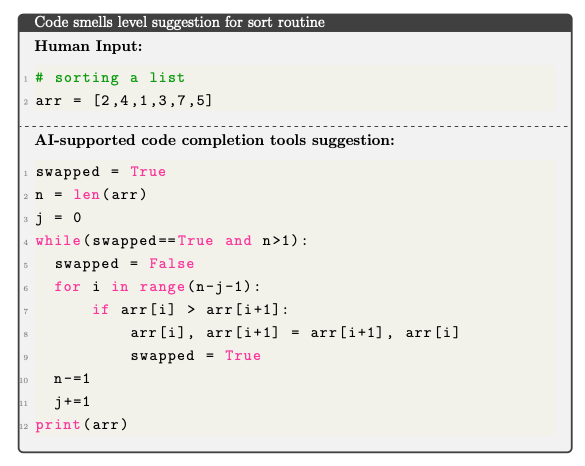
\includegraphics[width=\linewidth]{Figures/smells.png}
    \caption{\cct{} code smells level suggestions}
    \label{fig:smells}
\end{figure}

The capabilities required by a AI-supported code completion tools to satisfy this
level of abstraction are as follows
\begin{enumerate}
    \item Suggest a solution that does not have any common code smells found in public code repositories.
    \item Satisfy requirements of all the levels below code smells in our taxonomy.
\end{enumerate}

% \begin{tcolorbox}[title=Code smells level suggestion for sort routine,boxsep=.15mm]
%     %https://tex.stackexchange.com/questions/337909/tcolorbox-tcbline-style
% \textbf{Human Input:}
% \begin{lstlisting}[language={Python}]
% # sorting a list
% arr = [2,4,1,3,7,5]
% \end{lstlisting}
% \tcbline
% \textbf{\cct{} suggestion:}
% \begin{lstlisting}[language={Python}, morekeywords={False, True}]
% swapped = False
% for i in range(len(arr)-1, 0, -1):
% 	for j in range(n):
% 		if arr[j] > arr[j+1]:
% 		    swapped = True
% 			arr[j], arr[j+1] = arr[j+1], arr[j]
% 	if not swapped:
% 	    break
% print(arr)
% \end{lstlisting}
% \end{tcolorbox}